% Appendix B

\chapter{El Modelo Relacional Gompertz de Fertilidad de Brass} % Main appendix title

\label{AppendixB} % For referencing this appendix elsewhere, use \ref{AppendixA}

El modelo relacional Gompertz de fertilidad de Brass es directamente análogo al modelo de mortalidad logit (también de Brass). Al igual que con este modelo, el modelo relacional de fertilidad hace uso de un programa de fertilidad estándar que se linealiza (es decir, se convierte en una línea -casi- recta) por medio de una función matemática.

Esta línea recta puede transformarse luego en cualquier otra línea recta cambiando su pendiente y punto de intercepción, y luego volver a convertirla en un programa de fertilidad, aplicando la anti-función utilizada para linealizar el programa estándar.\\

Brass identificó que la función de Gompertz describe bien el patrón de fertilidad acumulada, \textit{F(x)}, en una población. Esta función es sigmoidal (en forma de s) y ligeramente inclinada hacia la derecha, capturando así la presunta forma de una curva de fertilidad, \textit{f(x)}, presente en la mayoría de las poblaciones.\\

Con un programa de fertilidad estándar con una TFR\footnote{\textit{Total Fertility Rate:} la Tasa Total de Fertilidad es el número medio de hijos que una mujer tendría si sobreviviera hasta el final de la edad reproductiva.} de 1, \textit{f\textsubscript{s}(x)}, \textit{F\textsubscript{s}(x)} es la proporción de TFR alcanzada por la edad \textit{x} en el programa de fertilidad estándar. El programa de fertilidad estándar original fue construido por Heather Booth (1984), una estudiante de Brass.\\

\textbf{Formulación matemática del modelo:}\\

\noindent La transformación que linealiza \textit{F\textsubscript{s}(x)} a números reales entre 0 y 1 es el logaritmo natural doble: $$Y_{s}(x)=-ln[-ln F_{s}(x)]$$ Transformaciones lineales de \texit{Y\textsubscript{s}(x)} $$Y_{m}(x)=\alpha + \beta Y_{s}(x)$$ producen transformaciones de los esquemas de fertilidad modelizados, tal y como los logits se derivan de los estándares.\\
La transformación inversa que convierte el modelo \textit{Y\textsubscript{s}(x)} de nuevo en la fertilidad acumulada proporcional, es el doble exponencial (la doble exponencial se conoce universalmente como la función de Gompertz, después de que el actuario Benjamin Gompertz, la utilizara para describir la mortalidad por vejez). $$\widetilde{F}_{m}(x)=e^{-Y_{m}(x)}$$ $$=exp[-exp{-Y_{m}(x)}]$$ Para convertir estos valores acumulados de fertilidad proporcionales (o normalizados) en valores de fertilidad acumulados, se multiplican por el modelo TFR requerido: $$F_{m}(x)=T\cdot\widetilde{F}_{m}(x)$$

\textbf{Esquemas de fertilidad derivados del modelo de fertilidad relacional de Gompertz de Brass:}\\

\noindent Por lo tanto, el modelo de Brass tiene tres parámetros: \textit{T}, $\alpha$ y $\beta$, donde:\\

\textbullet\ $T$, controla el nivel de fertilidad.

\textbullet\ $\alpha$, determina la ubicación de la distribución de la fertilidad. Debido a que la distribución estándar está sesgada, las medidas de ubicación (particularmente el modo) se ven afectadas por $\beta$, pero en menor medida que por $\alpha$.

\textbullet\ $\beta$, determina la expansión (o propagación) de la distribución.\\

En la siguiente figura hemos simulado el modelo para los valores de los parámetros $\alpha=0.15$, $\beta=0.85$ y una TFR = 5 (curva de color azul) y se muestra, para comparar, con el modelo estándar de parámetros  $\alpha=0$, $\beta=1$ y TFR = 3 (curva de color verde):

\begin{figure}[!ht]
\centering
\hspace*{-0.1cm}
\fbox{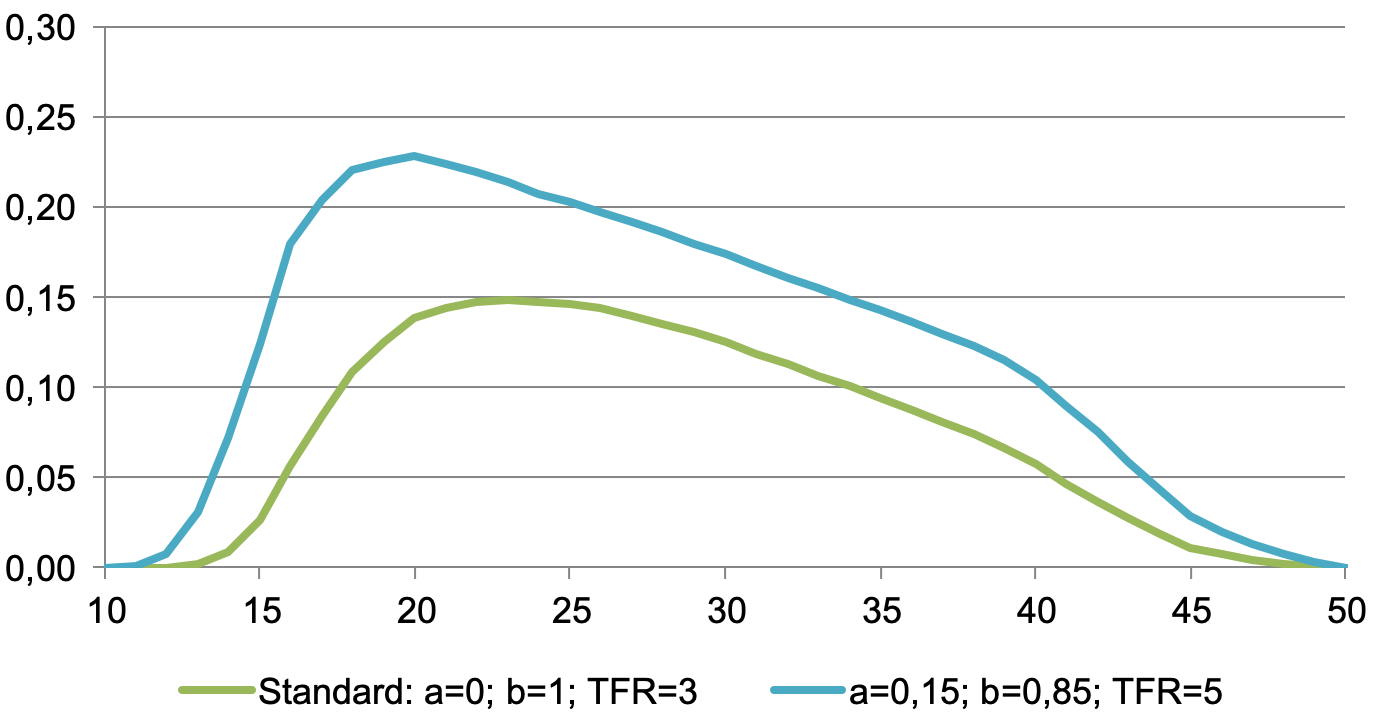
\includegraphics[scale=0.45]{Apendices/gompertz.png}}
\caption{Simulación en Excel del modelo relacional Gompertz de fertilidad de Brass}\\
\end{figure}

La capacidad de ajustar la distribución de la distribución proporciona el grado extra de flexibilidad que faltaba en el modelo logit de Brass. El modelo de fertilidad relacional Gompertz es mucho más fácil de ajustar a los datos observados que cualquiera de los modelos de Romaniuk, Hadwiger o Coale-Trussell. Todo lo que hay que hacer es establecer las constantes en la relación lineal entre la función $Y_{s}(x)$ observada y estándar; esto se puede hacer por mínimos cuadrados o gráficamente, según la precisión requerida. También se ajusta a la mayoría de los datos de fertilidad observados también o mejor que los otros modelos, aunque tiene menos parámetros. El estándar ha sido construido para representar la acumulación inicial de fertilidad de manera realista, y si se requiere una mayor flexibilidad o un ajuste más estrecho para un conjunto de datos en particular, se puede elegir un estándar diferente de datos empíricos o de otro modelo. Sin embargo, solo el estándar Booth ha encontrado un uso y una aplicación generalizados.

Una aplicación particularmente útil del modelo relacional Gompertz es la corrección y el ajuste de los datos de fertilidad, que está sujeto a los tipos de errores que generalmente se encuentran con los datos recopilados en los censos de los países en desarrollo. Como antes, el ajuste de los modelos de Gompertz relacionales a los datos de fertilidad observados requiere la estimación de los parámetros $\alpha$, $\beta$ y la tasa de fertilidad total (TFR).